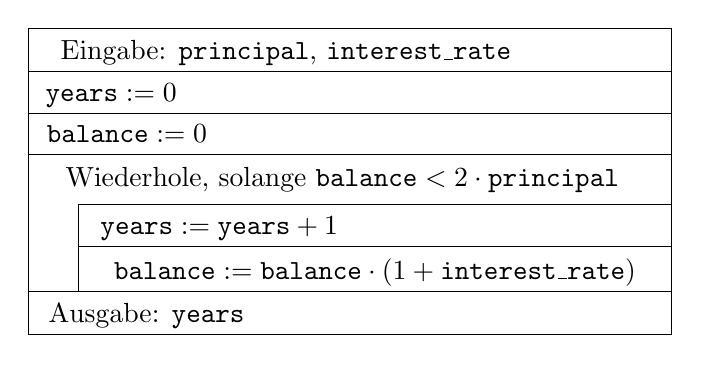
\begin{tikzpicture}
    \draw (0pt,0pt) rectangle (232.56723pt, -15.60416pt);
    \node at (93.12139pt, -9.018745000000001pt) {Eingabe: \texttt{principal}, \texttt{interest\_rate}};
    \draw (0pt,-15.60416pt) rectangle (232.56723pt, -30.66082pt);
    \node at (29.930015pt, -24.349155pt) {$\texttt{years} := 0$};
    \draw (0pt,-30.66082pt) rectangle (232.56723pt, -45.71748pt);
    \node at (35.6787pt, -38.18915pt) {$\texttt{balance} := 0$};
    \draw (0pt,-45.71748pt) rectangle (232.56723pt, -95.02413pt);
    \node at (4.0pt, -70.370805pt) {};
    \node at (113.45384pt, -54.736225pt) {Wiederhole, solange $\texttt{balance} < 2 \cdot \texttt{principal}$};
    \draw (18.03749pt,-63.75497pt) rectangle (232.56723pt, -78.81163000000001pt);
    \node at (69.03085999999999pt, -72.499965pt) {$\texttt{years} := \texttt{years} + 1$};
    \draw (18.03749pt,-78.81163000000001pt) rectangle (232.56723pt, -95.02413000000001pt);
    \node at (125.30236pt, -88.28662500000002pt) {$\texttt{balance} := \texttt{balance} \cdot (1 + \texttt{interest\_rate})$};
    \draw (0pt,-95.02413pt) rectangle (232.56723pt, -110.62828999999999pt);
    \node at (42.73549pt, -104.04287500000001pt) {Ausgabe: \texttt{years}};
\end{tikzpicture}
